\documentclass[a4paper,11pt]{article}
\usepackage[a4paper, total={6.6in, 9.7in}]{geometry}
\usepackage{graphicx}
\graphicspath{ {./images/output/} }
\usepackage{caption}
\usepackage[english]{babel}
\usepackage{titling}
\usepackage{float}
\usepackage{amsmath}
\usepackage{minted}
\usepackage{multicol}
\usepackage{array}
\usepackage{setspace}
\usepackage{placeins}
\usepackage{parskip}

% \usepackage{lipsum}

\title{Experiment 3 \\
    \textbf{Experimental Observation of Various Features of an ECG Signal Collected from PhysioNet Public Dataset}}
\author{}
\date{}

\pagenumbering{gobble}
\begin{document}
\vspace*{\fill}
\begin{center}

    \emph{Heaven's Light is Our Guide} \\
    \textbf{Rajshahi University of Engineering and Technology} \\

    \begin{figure}[H]
        \centering
        
\includegraphics[scale=.34]{images/RUET_logo.png}
        \label{fig:ruet_logo}
    \end{figure}
    \vspace{5mm}

    \textbf{Course Code}\\
    ECE 4144\\
    \vspace{3mm}
    \textbf{Course Title}\\
    Biomedical Engineering Sessional

    \vspace{5mm}
    \textbf{Experiment Date:} {August 06, 2025},\\
    \textbf{Submission Date:} {August 13, 2025}\\

    \vspace{5mm}
    \textbf{Lab Report 3: \\
        Experimental Observation of Various Features of an ECG
        Signal Collected from PhysioNet Public Dataset}

    \vspace{15mm}

    \begin{tabular}{c|c}
        \textbf{Submitted to} & \textbf{Submitted by} \\
        Md Mayenul Islam      & Md. Tajim An Noor     \\
        Assistant Professor   & Roll: 2010025         \\
        Dept of EEE, Ruet     &                       \\
    \end{tabular}

\end{center}
\vspace*{\fill}


\pagebreak
\maketitle

\vspace{-6em}

\section*{Objectives}
\begin{itemize}
    \item Measure key ECG features (RR, PP, PR intervals) using a PhysioNet dataset.
    \item Relate these intervals to heart rate and cardiac function.
\end{itemize}

\vspace{-.8em}

\section*{Theory}
An electrocardiogram (ECG) records the heart's electrical activity~\cite{ecgbook}. Key features include the P wave, QRS complex, and T wave.

Important intervals:
\begin{itemize}
    \item \textbf{RR Interval}: Time between R-wave peaks; used to calculate heart rate.
    \item \textbf{PP Interval}: Time between P-wave peaks; reflects atrial rhythm.
    \item \textbf{PR Interval}: From P-wave onset to QRS start; indicates atrioventricular conduction.
\end{itemize}

Heart rate (HR) is calculated from the RR interval~\cite{ecgbook}:
\[
    \text{Heart Rate (bpm)} = \frac{\text{Number of R-peaks}}{\text{Time (s)}} \times 60
\]

\vspace{-.8em}

\section*{Dataset Description}
This experiment uses the MIT-BIH Arrhythmia Database from PhysioNet, which contains 48 half-hour, two-channel ECG recordings from 47 subjects~\cite{mitbih}.

\textbf{Key details:}
\begin{itemize}
    \item \textbf{Sampling Frequency:} 360 Hz
    \item \textbf{Annotations:} $\sim$110,000
    \item \textbf{Subjects:} 60\% inpatients, 40\% outpatients
\end{itemize}

Record 100 was analyzed, including files: \texttt{100.atr} (annotations), \texttt{100.dat} (ECG data), \texttt{100.hea} (metadata), and \texttt{100.xws} (extra waveform data).

\vspace{-.8em}

\section*{Tools Used}
\begin{itemize}
    \item \textbf{MATLAB}: For ECG signal processing and analysis.
    \item \textbf{WFDB Toolbox}: To access and handle PhysioNet data in MATLAB.
\end{itemize}

\vspace{-.8em}

\section*{ECG Signal Analysis: MATLAB Implementation}
The MATLAB code below reads ECG data from the MIT-BIH Arrhythmia Database, plots a segment, and calculates heart rate and key intervals:

\inputminted[fontsize=\small,breaklines, linenos]{matlab}{assets/ecg.m}

\vspace{-.8em}

\subsection*{Output}
\begin{verbatim}
    Heart Rate (bpm): 78.00
    Mean R-R Interval (samples): 288.50
    Mean R-R Interval (seconds): 0.8014
    Mean P-P Interval (samples): 289.00
    Mean P-P Interval (seconds): 0.8028
\end{verbatim}

\vspace{-.8em}

\subsection*{Annotated ECG Segment}
\begin{figure}[H]
    \centering
    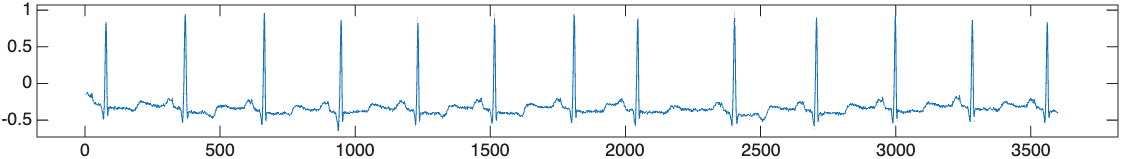
\includegraphics[width=\textwidth]{ecg.png}
    \caption{ECG segment with R- and P-peaks.}
\end{figure}

\vspace{-.8em}

\section*{Result \& Discussion}
The analysis yielded:
\begin{itemize}
    \item \textbf{Heart Rate:} 78 bpm
    \item \textbf{Mean R-R Interval:} 288.5 samples ($0.80$ s)
    \item \textbf{Mean P-P Interval:} 289.0 samples ($0.80$ s)
\end{itemize}
These results, obtained using MATLAB and WFDB Toolbox, confirm accurate peak detection and fall within normal adult ranges.
The close agreement between RR and PP intervals indicates a regular sinus rhythm in the analyzed ECG segment.

\bibliographystyle{IEEEtran}
\renewcommand{\bibname}{References}
\addcontentsline{toc}{section}{References}
\bibliography{ref}

\end{document}
